\chapter{Transport Calculations with \wannier\ }\label{ch:transport}

By setting $\verb#transport#=\verb#TRUE#$, \wannier\ will calculate
the quantum conductance and density of states of a one-dimensional
system. The results will be written to files \verb#seedname_qc.dat#
and \verb#seedname_dos.dat#, respectively.

The system for which transport properties are calculated is determined
by the keyword \verb#transport_mode#.

\section{\tt transport\_mode = bulk}

Quantum conductance and density of states are calculated for a perfectly
periodic one-dimensional conductor. If $\verb#tran_read_ht#=\verb#FALSE#$
the transport properties are calculated using the Hamiltonian in the Wannier 
function basis of the system found by \wannier. Setting 
$\verb#tran_read_ht#=\verb#TRUE#$ allows the user to provide an 
external Hamiltonian matrix file {\tt seedname\_htB.dat}, from which
the properties are found. See Section~\ref{sec:post-p} for more details of 
the keywords required for such calculations.

\section{\tt transport\_mode = lcr}

Quantum conductance and density of states are calculated 
for a system where semi-infinite, left and right leads
are connected through a central conductor region. This is known 
as the \emph{lcr} system.
Details of the method is described in Ref. \cite{Nardelli}.

In \wannier\ two options exist for performing such calculations: 
\begin{itemize}
\item If $\verb#tran_read_ht#=\verb#TRUE#$ the external Hamiltonian 
files {\tt seedname\_htL.dat, seedname\_htLC.dat, seedname\_htC.dat, 
seedname\_htCR.dat, seedname\_htR.dat} are read and used to compute 
the transport properties. 
\item If $\verb#tran_read_ht#=\verb#FALSE#$, then the transport
calculation is performed automatically using the Wannier functions as a
basis and the 2c2 geometry described in Section~\ref{sec:2c2}.
\end{itemize}

\section{Automated lcr Transport Calculations: The 2c2 Geometry}
\label{sec:2c2}

Calculations using the 2c2 geometry provide a method to calculate the
transport properties of an lcr system from a single \wannier\ calculation.
The Hamiltonian matrices which the five external files provide in the 
$\verb#tran_read_ht#=\verb#TRUE#$ case are instead built from the 
Wannier function basis directly. As such, strict rules apply to the system geometry, 
which is shown in Figure~\ref{fig:2c2}. These rules are as follows:
\begin{itemize}
\item Left and right leads must be identical and periodic.
\item Supercell must contain two principal layers (PLs) of lead on the left,
a central conductor region and two principal layers of lead on the right.
\item The conductor region must contain enough lead such that the
disorder does not affect the principal layers of lead either side.
\item A single k-point (Gamma) must be used.
\end{itemize}

\begin{figure}[h]
\centering
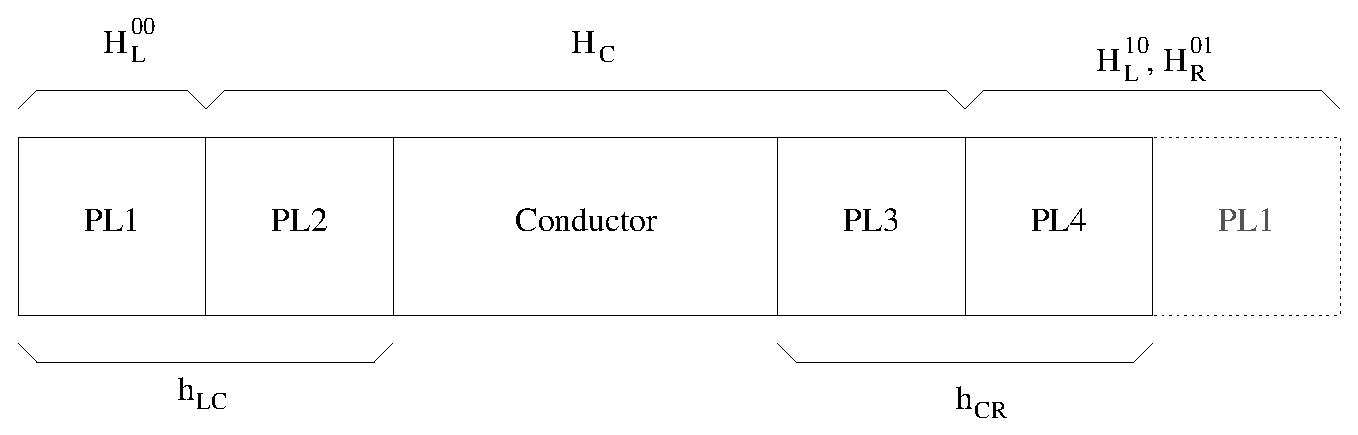
\includegraphics[height=4cm]{lcr_2c2}
\caption{Schematic illustration of the supercell required for 2c2
lcr calculations, showing where each of the Hamiltonian matrices
are derived from. Four principal layers (PLs) are required plus the
conductor region.}
\label{fig:2c2}
\end{figure}

In order to build the Hamiltonians, Wannier  functions are first 
sorted according to position and then consistent parities are enforced.
Therefore the following are also required:
\begin{itemize}
\item The number of Wannier functions in a principal layer, 
\verb#tran_num_ll#.
\item The number of unit cells in one PL of lead
\verb#tran_num_cell_ll#.
\item The \verb#UNKp.s# file.
\end{itemize}

Further parameters related to these calculations are 
\verb#tran_group_threshold# and \verb#tran_wf_threshold#.

Examples of how 2c2 calculations are performed can be found 
in the \wannier\ Tutorial.
